\documentclass[a4paper,5pt]{article}
\usepackage{tikz}
\usetikzlibrary{arrows,positioning} 


%\begin{document}


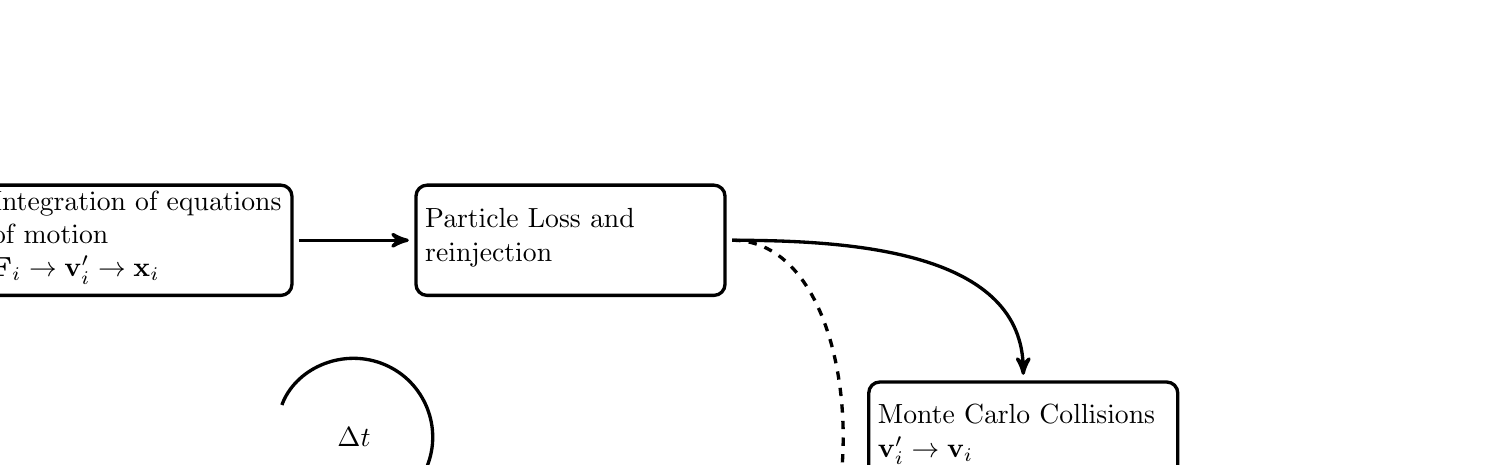
\begin{tikzpicture}[node distance=5cm,font=\normalsize,auto]
\tikzset{
    %Define standard arrow tip
    >=stealth',
    %Define style for boxes
    punkt/.style={
           rectangle,
           rounded corners,
           draw=black, very thick,
           text width=10.5em,
			  text height=0.5em,
			  minimum width=2.5cm,
           minimum height=1.4cm,
			  text badly ragged},
    % Define arrow style
    pil/.style={
           ->,
           very thick,
           shorten <=2pt,
           shorten >=2pt,}
}
	\path[use as bounding box,anchor=mid west] (-3.6in,0) rectangle (3.6in,5.2cm);

 	\node[shift={(-5cm,0cm)}] (dtcenter) at (0,0) {$\Delta t$};
	\node[shift={(160:1cm)}] (circstart) at (dtcenter) {};
	\draw[pil] (circstart) arc (160:-160:1cm);
 %nodes

 	\node[punkt,shift={(-2.75cm,2.5cm)}] (padvnc) at (dtcenter) {Integration of equations of motion\newline $\mathbf{F}_i \rightarrow \mathbf{v}_i' \rightarrow \mathbf{x}_i$};

 	\node[punkt,shift={(2.75cm,2.5cm)}] (ploss) at (dtcenter) {Particle Loss and reinjection};

	\node[punkt,shift={(8.5cm,0)}] (collide) at (dtcenter) {Monte Carlo Collisions\newline $\mathbf{v}_i' \rightarrow \mathbf{v}_i$};

	\node[punkt,shift={(2.75cm,-2.5)}] (c2mesh) at (dtcenter) {Interpolation of particled to mesh\newline $(\mathbf{x}_i\mathbf{v}_i) \rightarrow \rho_j$};

	\node[punkt,shift={(-2.75cm,-2.5)}] (psolve) at (dtcenter) {Integration of field equations\newline $\rho_j \rightarrow \mathbf{E}_j$};

	\node[punkt,shift={(-6.5cm,0)}] (mesh2p) at (dtcenter) {Interpolation of fields to particles\newline $\mathbf{E}_j \rightarrow \mathbf{F}_i$};

	\path (padvnc.east) edge[pil] (ploss.west);
	\path (ploss.east) edge[very thick,dashed,out=0, in=0,shorten <=2pt,shorten >=2pt,] (c2mesh.east);
	\path (ploss.east) edge[pil,out=0, in=90] (collide.north);
	\path (collide.south) edge[pil,out=-90, in=0] (c2mesh.east);
	\path (c2mesh.west) edge[pil] (psolve.east);
	\path (psolve.west) edge[pil,out=180,in=-90] (mesh2p.south);
	\path (mesh2p.north) edge[pil,out=90,in=180] (padvnc.west);
	

\end{tikzpicture}

\end{document}

%%% Local Variables:
%%% mode: latex
%%% TeX-master: t
%%% End:
